\documentclass{article}
\usepackage[utf8]{inputenc}
\usepackage{amsmath}
\usepackage{amssymb}
\usepackage{amsthm}
\usepackage{graphicx}


\newtheorem{theorem}{Theorem}
\newtheorem*{definition}{Definition}
\newtheorem*{remark}{Remark}
\newtheorem*{claim}{Claim}
\newtheorem*{lemma}{Lemma}

\title{Random Arrangements in Surf Competition Judging: Testing Exchangeability}
\author{Jojo Aboaf and Marty Wells}
\date{June 30th 2021}

\begin{document}
\maketitle
\tableofcontents

\begin{abstract}
We have collected the most complete data set on international surf competition publicly available.
We present an empirical method for analyzing arrangement data in order to test for Nationality bias in International Surf Competitions. 
We present a test for exchangeability  an empirical method for analyzing arrangement data in order to test for Nationality bias in International Surf Competitions. 

\end{abstract}
\section{Introduction}
Editing Notes: I don't know where this should go.
A wide range of non-performance based biases are documented and researched using various methods; for example, Price and Wolfers study own-race bias in NBA refereeing using [        ], [   ] and [  ] investigate nationality bias in synchronized swimming judging using [       ], and ordering bias of gymnastics judges. These are only a few examples in sports, but the social-cognitive underpinnings of biases are a key area of research in psychology and legal studies.

\section{Motivation}
Our goal in this paper is to construct a method to determine if judges have a tendency to give higher scores to surfers from their home countries compared to judges with nationalities different from the surfer. To achieve this we will identify the empirical distribution of arrangements of judges and test if this distribution is significantly different from its symmetric part. That is, 

Our focus will be on arrangements or partial arrangements of judges, which we will analyze "by match" and "by country". An arrangement is simply a sequence and a partial arrangement is a sequence of arrays. We define an array as an unordered collection of things (in our case, country labels), and any thing may occur with any multiplicity in an array.

This algebraic structure of a partial arrangement was motivated by high proportion of panels with multiple judges from the same country and the high proportion of partial arrangements. More broadly, the literature on ordered statistics and rankings is focused on the case where each data point consists of a full or partial order on a set of distinct labels (\cite{LebMao08},\cite{FliVer93}).

\begin{table*}
\caption{Orderability and Multiplicities in the Data }
\label{OrderAndMultOfData}
\begin{center} \begin{tabular}{|c|c|c|c|}
\hline
 & Totally Ordered & Not Totally Ordered & Row Sum  \\ 
\hline
5 Distinct Countries & 248 (0.0179)  & 2830 (0.2040) & 3078 (0.2219)  \\
5 Non-Distinct Countries & 891 (0.0642)  & 9903 (0.7139) & 10794 (0.7781) \\
\hline
Col Sum  & 1139 (0.0821) & 12733 (0.9179)&  13872 (1.0000)\\
\hline
\end{tabular} \end{center}
\end{table*}

Our ideas were inspired by those of Lebanon and Mao in \cite{LebMao08} and Moyal in \cite{Moyal62}. We have also made extensive use of the ideas in Persi Diaconis' book, Group Representations in Probability and Statistics, and direct the interested reader there \cite{Diaconis88}. Together, they provide a comprehensive approach to data which falls into the top row.

The surfing data evidently requires an approach that is suited to handle labels occurring with multiplicity, and particularly the case where these labels are not totally ordered. To adress these needs, we will present two approaches. The first will treat an ordered partition of a judges as a vector-partition of the vector whose coordinates correspond to the number of judges from each country. This will omit some structure, leaving hypothesis testing procedures less enlightening. The second, is inspired by Moyal's approach to point processes when a population consists of distinguishable or indistinguishable members. We provide a similar, more explicit, algebraic construction which will account for multiplicities arising from unordered observations. In doing so, we will find the remaining parts of the table to be important special cases.

More broadly, the methodology and associated computation presented is applicable to any situation in which the unit of analysis is a sequence of arrays of labels. With the surf-competition data, we consider the order statistic of a panel, which is a sequence where the ith entry is an array containing the nationalities of the judges that gave the ith highest score. This means that order statistic is of a random length, depending on the number of distinct scores given my the judges.

In applied settings we cannot expect labels to occur without multiplicity or be totally ordered or be of uniform length.

%A "matching" judge is one that has the same nationality as the surfer being scored, and a non-matching judge is a judge with a different nationality than the surfer being scored. This reduces judges for a given wave to a binary variable. It the more general "by country" case, judges are identified by their nationality, which leaves a random arrangement
%To analyze the orders of judges by nationality, it suffices to analyze the orderings of the set $C := \{AUS, BRA, FRA, \dots, ZAF\}$, which is the set of all nationalities of judges who scored any wave from 2017 to 2019.
% Though we are not concerned with the arrangement of the elements of $x^i$ for any $i$, we cannot consider $x^i$ to be a set in general because it must accommodate observations that have multiple judges from the same country in same block. This distinguishes the surf-judging data and the statistical approach from what is typically considered in random partition literature.

\section{Background: Professional Surfing}

\subsection{Overview}
The WSL Championship Tour (CT) is a series of events in which surfers are allocated points based on their placement in each of the constituent events and the surfer with the most points at the end of the season is crowned the WSL CT champion. While event formats and point allocation mechanisms have changed, surfers that advance though more rounds of an event are allocated more points. In addition to Championship Tour (CT), the WSL operates multiple Qualifying Series (QS): QS10000, QS6000, QS3000, QS1500, and QS1000. The number associated with a certain qualifying series indicates the number of points awarded to the winner of one of its constituent events. The specific breakdown of points awarded for various placement at QS events can be found in Appendix B of the WSL Rule Book.

In this paper, we focus on the 2017, 2018, and 2019 seasons of the Men’s Championship Tour because it offers the fullest set of waves that list judge scores along with their nationality. This study uses 15,990 waves surfed in 2017, 2018, and 2019 seasons to empirically analyze the role of judge nationalities in the Men's Championship Tour.
\subsection{Format}
Each year, the 32 highest ranked (short board) surfers are invited to participate in the”Championship Tour” (CT), which consists of 11 surf competitions in 7 different countries.Each competition has 7 rounds, each consisting of 1 to 16 heats, and each heat has 2 to 3 surfers. Within a heat, a surfer may attempt to ride any number of waves, but their final heat score is the sum of their two highest scoring waves. The surfer with the highest heat score places 1st in the heat, the surfer with the next highest heat score places 2nd in the heat. If there are 3 surfers, the surfer with the third highest heat score will place 3rd in the heat.
\subsection{Data}
The World Surf League (WSL) holds a variety of tours or series' at the professional or amateur level (similar to how the MLB organizes A, AA, and AAA baseball). A "tour" or "series" is a sequence of events. Tours have seasons that typically last no more than 365 days and they tend to be contained within one calendar year (i.e. there is a 2019 season of a tour).
We collected some rich data on the 2017, 2018, and 2019 seasons of the Men's Championship Tour (CT). This is the highest level of competitive short board surfing in the world. Each season typically consists of 10 or 11 surf competitions, which are called "events". The format of an event has changed throughout our sample, but they are fairly similar. An event consists of 7 or 8 rounds, and within each round there are some number of heats. A "heat" is the level where direct competition between athletes takes place. Typically, there are 2 or 3 surfers in a heat and the duration is 22 or 35 minutes. During a heat, a surfer may attempt to ride any number of waves. Anytime a surfer rides a wave, they receive a non-zero score determined by the scores of a judging panel. There are 5 judges on a panel for any given heat. They are visually separated and do not discuss scores. When a surfer takes a wave, they each observe the ride and write down a score which is some number between 0.1 and 10.0 and it is precise up to the tenths place. The highest and lowest scores given by the panel are dropped, and the surfer receives the mean of the 3 remaining scores for their ride, this is called the "wave score". These are rounded to 2 digits. At any given point in a heat, a surfer has a "heat score", which is the sum of their two highest scores, and simply the sum of their scores if they have surfed 0, 1, or 2 waves. When the time allocated for a heat elapses, a horn will sound, and the surfer with the highest heat score is awarded first place, the surfer with the second highest score is awarded second, and so on, if there are more surfers. The result of finishing a heat in a particular place depends on the round.  Each round has a rule that determines which surfers advance, and what (round,heat) they advance to.  Surfers that do not advance ”exit” the event and are given some number of points. (The longer a surfer stays in an event, the more points they are allocated at an exit). The 2019 event format is depicted below.
THOUGHT: Maybe i should add number of points to the exists.
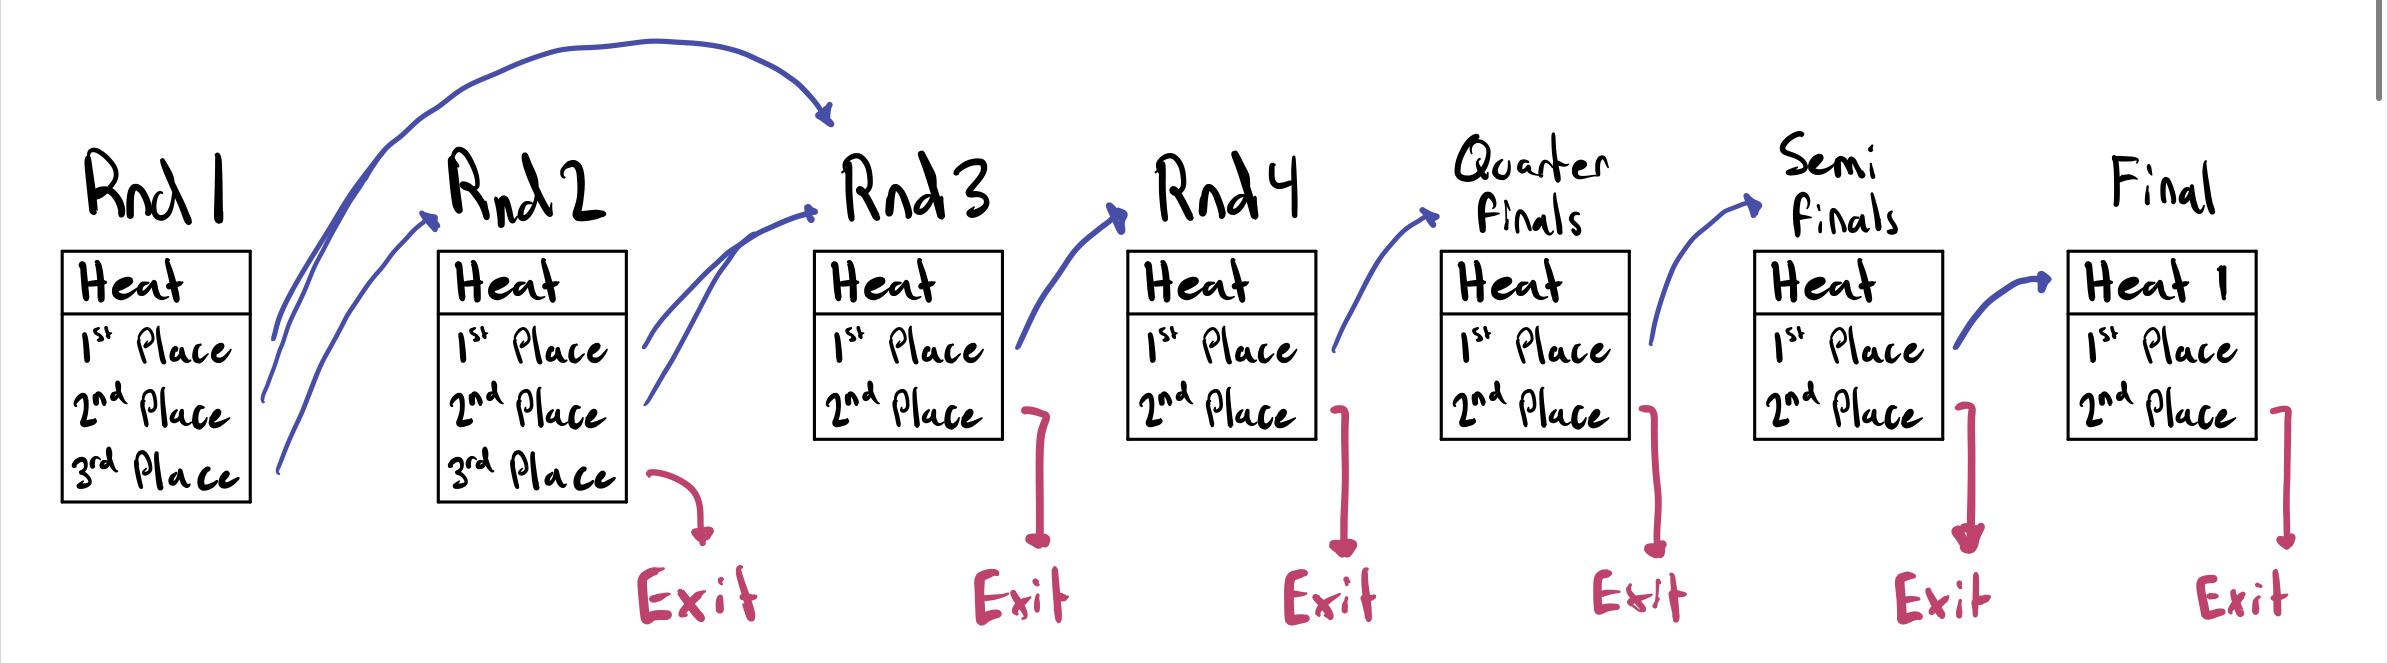
\includegraphics[width=\textwidth]{./visuals/2019EvtFormat.jpeg}

\subsection{Intricacies of the Data Generating Process}
The motivation for this publication is not only to present some analytical statistical methods to panel data but also to describe the intricacies of (this) surfing data. Explicitly, we have focused our efforts on one specific part of this data, the panel. There are many other aspects of this data that make it interesting from a statistical perspective.

\subsubsection{Notions of “Origin”, “Country”, or “Nationality”}
When collecting nationality associated with a particular athlete or a judge’s score, we observed a set of labels. These were not limited to the following set of countries:
	{AUS,BRA, ESP, FRA, PRT, USA, ZAF, FJI, IDN, ITA, JPN, NZL}
The original fields on the world surf league website also included Hawaii, French Polynesia, and Basque Country. None of these are globally recognized as independent nations. Hawaii is a state contained in the United States, French Polynesia is collective of France, and Basque Country is autonomous community in Spain. There is a less strict view of nationality, and one’s particular definition may render all, some, or none of the 3 a nationality. “Origin” seems to be a more inclusive term to describe where someone comes from, or how they identify that for themselves.

The exact motivation for these non-Country labels is unclear. The rulebook states that no more than BLAH events should be held in one region and no more than 3 judges from any one country should be on the panel at once and it says … “ ”.
Regardless, we will present results for two sets of labels:
C = {AUS,BRA, ESP, FRA, PRT, USA, ZAF, FJI, IDN, ITA, JPN, NZL}
R = {AUS, BAS, BRA, ESP, FRA, HAW, PRT, USA, ZAF, IDN, ITA, JPN, NZL}
Methods presented do not require you have notion or another, merely that one is consistent in this belief. Conclusions may differ depending on ones preferred definition. We encourage the reader to select one of these as their forgoing definition and observe how this choice may lead to different conclusions.

Much of the 2017 panel data includes judge scores and omits some of the judge nationalities. This is not a result of the web scraping process, rather the information available on the WSL site. A ‘-1’ in a judge nationality field indicates it was not available is unknown. Precisely, ‘-1’ may be interpreted as “one of the elements of C or some other country”, and likewise with R.

\subsubsection{On the Ordering of Waves}
Each wave has a unique identifier, called a “Wave ID”. These were valuable when collecting information and aggregating across procedures. Additionally, wave score data for a particular wave may be found at:
	INSERT LINK HERE
Each wave surfed in the world surf league appears to have a Wave ID. Hence, the Wave IDs for the World Surf League Championship tour are not linearly ordered or increase inconstant multiple. The IDs are strictly increasing from heat to heat, I.e. if waveid1 < waveid2 then the wave given by waveid1 is in the same heat or prior heat to that of waveid2. 

Within an a particular heat, Wave IDs do not determine the order in which the waves were taken. However, the order determined by the Wave IDs may be considered as a close approximation. On one hand, assuming the waves occurred in the order of Wave ID is a close approximation to reality and wrong. Unfortunately, we cannot provide a quantitative estimate for how close this is to the true ordering of waves. 
	IT IS INTERESTING TO CONSIDER WHAT A QUANTITATIVE ESTIMATE WOULD EVEN LOOK LIKE.
On the other hand, taking waves within a heat to be exchangeable would be a poor reflection of the heat- that is- in our opinion. It is a regular practice of the amazing and vibrant surf commentators to replay waves from earlier in the heat in order to speculate if a recent wave, that has yet to be scored, will receive a score higher or lower than a prior wave. That is, they assume judges are consistent with their scoring, i.e. inferior rides receive lower scores, equivalent rides receive equivalent scores, and superior rides receive higher scores.
This is an assumption of theirs which is up to personal interpretation. I, a surfer, and someone who watches surfing, thinks this is roughly appropriate. Another possible heat level dynamic to make note of is “score taming” for rides early in a heat. Precisely, the forgoing belief (also mentioned by the commentators) is that judges will resist giving especially high scores or 10s early on in a heat in case another ride occurs later one which must be given a sufficient premium over prior scores.

On Priority:

On Interference Calls:

On Judge Scores:

After the long process of scraping, cleaning, and validating the data, we set out to perform some basic analyses.

\section{Preliminary Analysis}
Our goal is to determine if judges have a tendency to give higher scores to surfers that share their same nationality.

The straight forward approach is to test the differences in means between judges with the same nationality as the surfer and those with a different nationality. So we perform a hypothesis test where our hypotheses are:
\[ H_0: \mu_M  - \mu_{\neg M} = 0  \quad H_1: \mu_M -\mu_{\neg M} \neq 0 \]
And the test statistic is $ t = \frac{\bar{x}}{s/\sqrt{N}} $. Note that we are performing a one sample t-test on a series of data $(x_i)_{i=1}^N$ where $x_i := \mu_{M,i}  - \mu_{\neg M,i}$.  We'd like to call a panel for a wave our "statistical unit". This would be a lie. Not every panel is included in these tests because some panels have 0 Judges from the same country as the surfer riding the wave. In those cases the difference in means between Matching judges and Non-Matching judges looks like:
\[\frac{\sum_{j \in \text{Matching Judges}} score(j) }{|\{Matching Judges\}|} - \frac{\sum_{j \in\text{Non-Matching Judges}} score(j) }{|\{Non-Matching Judges\}|} = \frac{0}{0} - \frac{\sum_{j \in\text{Non-Matching Judges}} score(j) }{|\{Non-Matching Judges\}} \]
This is undefined. Nonetheless, we are only interested in the difference in means exactly when there is a match between at least one judge's nationality and the surfer's nationality. Carrying out this test we obtain a t-value of 6.71160420326186, thus under the null hypothesis the probability we obtain this sample is less than 0.001. This is when we would typically write "therefore, we would reject the null hypothesis". There is nothing fishy about this, however the picture isn't so compelling and this procedure doesn't seem to pass the scream-"the judges are biased in favor of surfers from their home country"-at-a-surf-competition test. The latter is certainly subjective. 

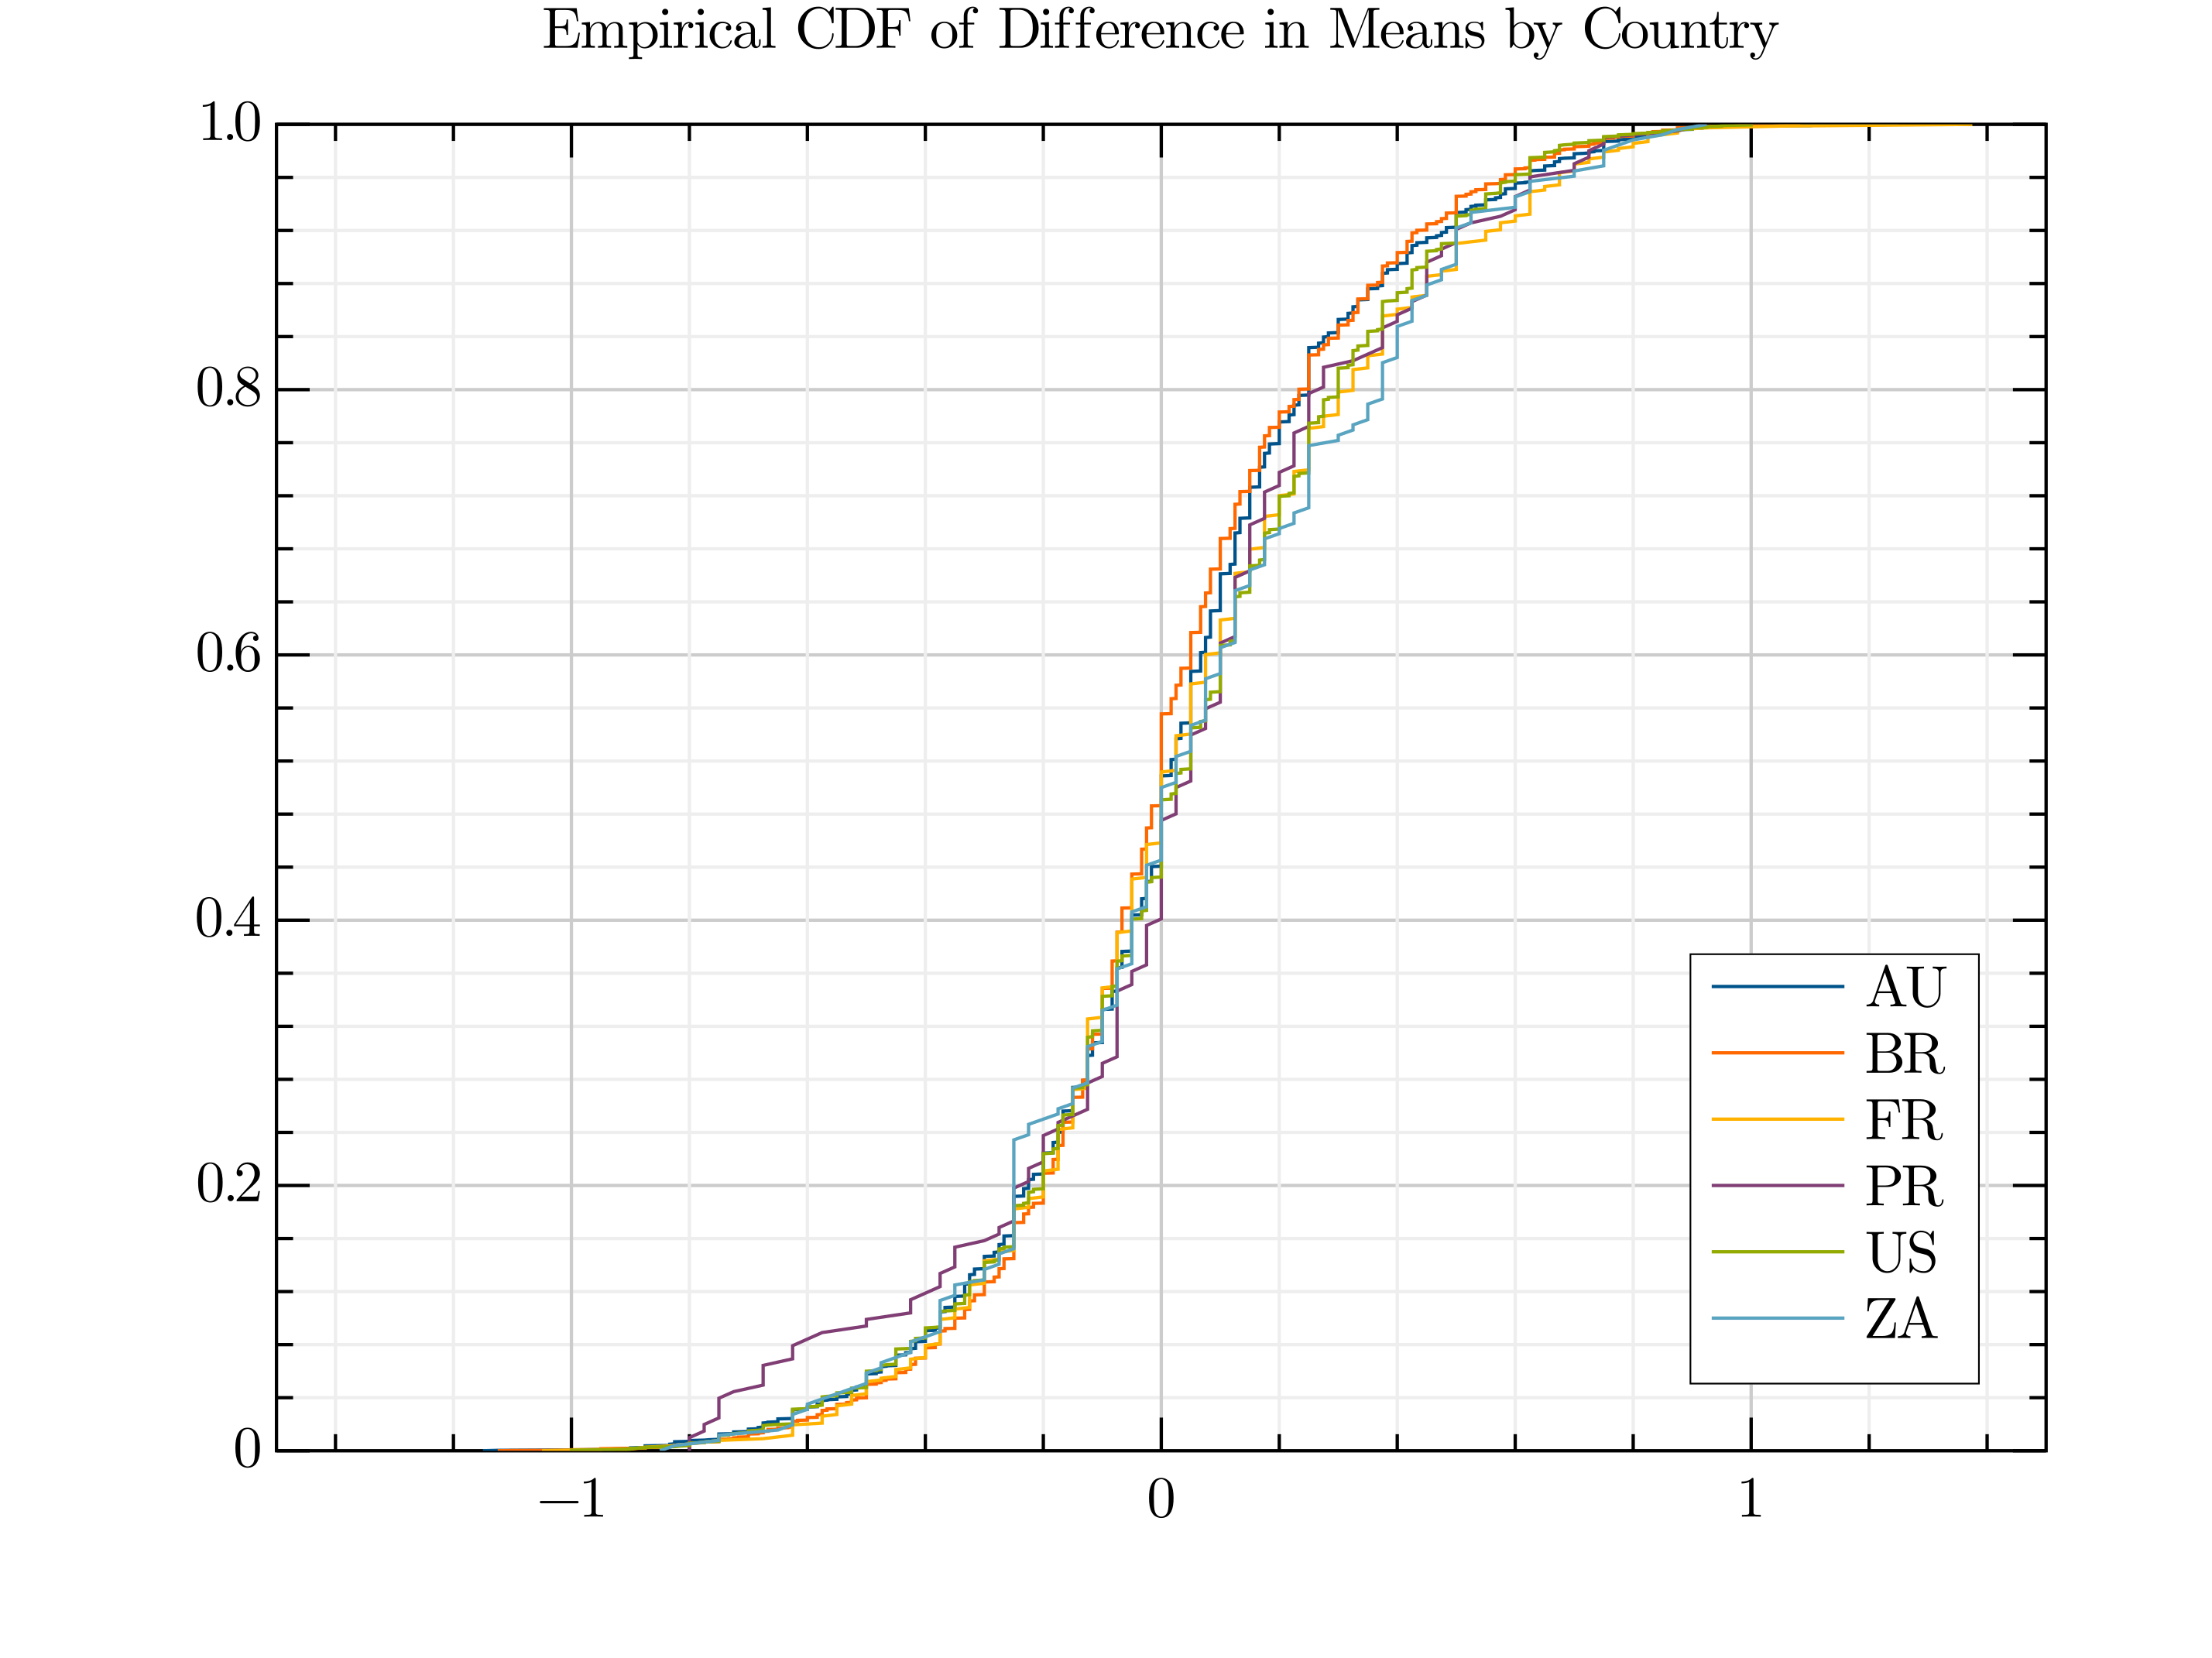
\includegraphics[width=\textwidth]{./visuals/ttests/CCtrue/EmpDiffInMeansCDF.png}
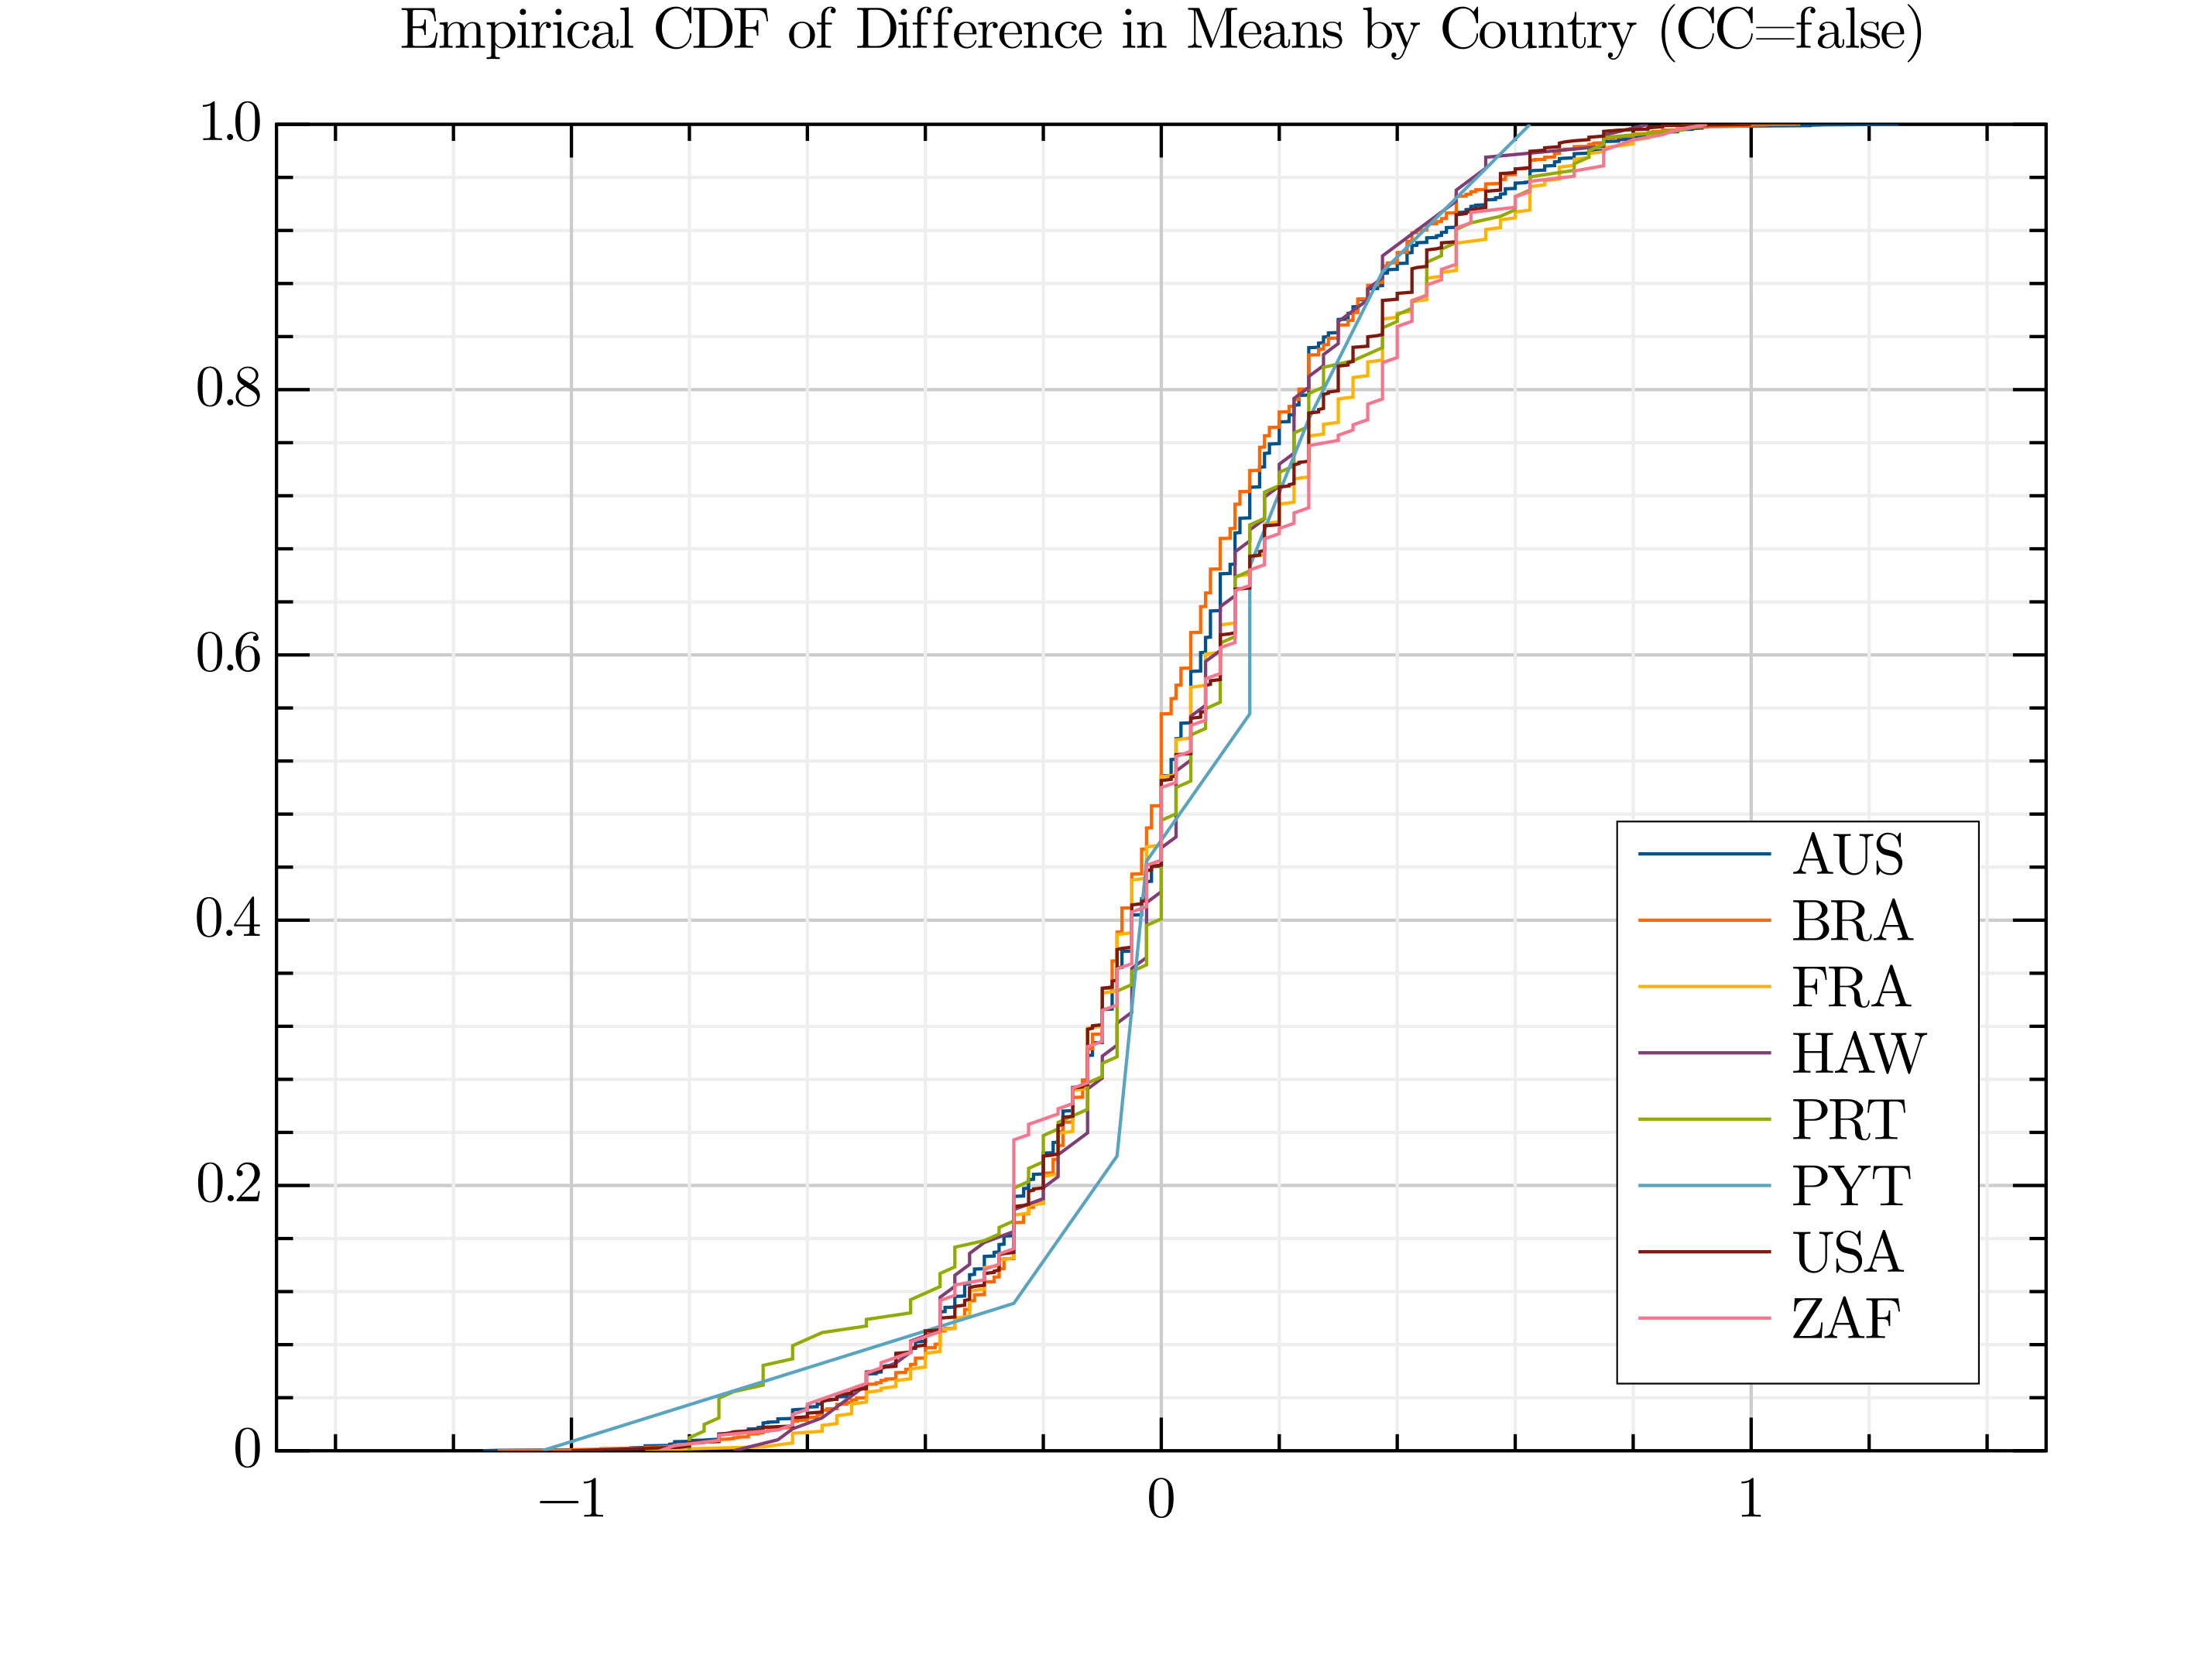
\includegraphics[width=\textwidth]{./visuals/ttests/CCfalse/EmpDiffInMeansCDF.png}

%\includegraphics[width=8cm]{./visuals/DiffInMeansCDFbyevent.png}
%\includegraphics[width=8cm]{./visuals/DiffInMeansCDFbyeventOrig.png}
%\includegraphics[width=8cm]{./visuals/DiffInMeansCDFbyathOrig.png}

\begin{table*}
\caption{Difference In Means t-test by Country (CC=True)}
\label{DiffInMeansttestsCCtrue}
\begin{center} \begin{tabular}{|c|c|c|c|c|c|c|} \hline
Country & AUS & BRA & FRA & PRT & USA & ZAF  \\ \hline
N & 3250 & 5234 & 769 & 203 & 2269 & 257  \\ \hline
$\hat{\mu}$ & 0.015 & 0.009 & 0.043 & 0.022 & 0.034 & 0.044  \\ \hline
t-val  & 2.703 & 2.302 & 3.632 & 0.854 & 5.082 & 2.072  \\ \hline
\end{tabular} \end{center}
\end{table*}

\begin{table*}
\caption{Difference In Means t-test by Country (CC=False)}
\label{DiffInMeansttestsCCfalse}
\begin{center} \begin{tabular}{|c|c|c|c|c|c|c|c|c|} \hline
Origin & AUS & BRA & FRA & HAW & PRT & PYT & USA & ZAF  \\ \hline
N & 3250 & 5234 & 682 & 122 & 203 & 10 & 1131 & 257  \\ \hline
$\hat{\mu}$ & 0.015 & 0.009 & 0.048 & 0.025 & 0.022 & 0.01 & 0.031 & 0.044  \\ \hline
t-val & 2.703 & 2.302 & 3.927 & 0.914 & 0.854 & 0.07 & 3.306 & 2.072  \\ \hline
\end{tabular} \end{center}
\end{table*}

\section{The Bare Bones Version}
This is the short version of what I'm trying to do. 
The Definitions and Notations are at the top and will be consistent throughout this section.

\section{Random Panel Approach}
A panel of judge-scores may be considered a matrix of counts of the number of judges from country c giving score s:
$ Q = \overbrace{\begin{bmatrix}
N_{(AUS,0.1)} & N_{(AUS,0.2)} & \dots & N_{(AUS,9.9)} & N_{(AUS,10.0)} \\
N_{(BRA,0.1)} & N_{(BRA,0.2)} & \dots & N_{(BRA,9.9)} & N_{(BRA,10.0)} \\
N_{(ESP,0.1)} & N_{(ESP,0.2)} & \dots & N_{(ESP,9.9)} & N_{(ESP,10.0)} \\
N_{(FRA,0.1)} & N_{(FRA,0.2)} & \dots & N_{(FRA,9.9)} & N_{(FRA,10.0)} \\
N_{(PRT,0.1)} & N_{(PRT,0.2)} & \dots & N_{(PRT,9.9)} & N_{(PRT,10.0)} \\
N_{(USA,0.1)} & N_{(USA,0.2)} & \dots & N_{(USA,9.9)} & N_{(USA,10.0)} \\
N_{(ZAF,0.1)} & N_{(ZAF,0.2)} & \dots & N_{(ZAF,9.9)} & N_{(ZAF,10.0)} \\
\end{bmatrix}}^{\text{Columns correspond to scores}}$, So $Q 1 = \begin{bmatrix}N_{AUS}\\ N_{BRA}\\N_{ESP}\\ N_{FRA}\\ N_{PRT}\\ N_{USA}\\N_{AUS}  \end{bmatrix}$ 
and $1^t Q = \begin{bmatrix} N_{0.1} & N_{0.2} & \dots & N_{9.9} & N_{10.0}\end{bmatrix}$.

Let Scores be the set of scores given by the judges, then:
\begin{itemize}
\item The first order statistic is $Z_{(1)} = Q[:,10*min(\text{scores})]$
\item The last order statistic is $Z_{(|scores|)} = Q[:,10*max(\text{Scores})]$
\item The order statistic of Q is: $Z = (Z_{(1)},\dots, Z_{(|\text{Scores}|)}) $
\end{itemize}

Each wave we observe a panel of judges. In its full generality, it is a 2 dimensional array. Like this:

We can read off all of the information we want from this. The entry in the $r$th row and $i$th corresponds to the number of judges from origin r, that gave score i. Technically, the judges gave a score of i/10, but nothing is lost, mathematically, by considering this as some integer out of 100. Perhaps there is a psychological effect?

This conception of a panel is possible because there are a finite number of values a judge may give a surfer for their efforts. So it is quite strait forward to "bucket" the judges by the score they gave. These are the columns. Once we have a particular score in mind, we can see how many judges from each country gave that score. These are the rows in the column.

We can also carry out this "reading off" process in reverse order. Pick a country, and to see what scores judges from that country gave, move along the row and each entry corresponds to the number of judges from that country giving the score i/10.

If we look at one particular panel, there will be many zeros because we are observing t judges in an array with 7x100=700 entries. So at most we have 5/700 non-zero entries.

Conditioning on "which country judges are from" means removing the rows corresponding to countries not in that set. For example, in Round 1, Heat 1 of Gold Coast 2018, we can condition condition on the panel origins = {AUS,BRA,ESP,USA,ZAF}, and every wave in this heat will have a panel that is contained in this "shortend" table. 

Similarly, we can condition on the panel origins in Round 1 Heat 2 of Gold Coast 2018, they are {AUS,BRA,USA}, in which case our "shortened panel" will look like:

Even though in both heats we see panels of 5 judges, we can have panels that are "shorter" than 5 because there are panels where multiple judges are from the same country. The WSL caps the number of judges from any single origin at 3, so in theory we will always have a panel that has at least 2 columns. (Though this rule is stated in the rule book, it appears that in the Round 3 Heat 14 of the 2019 Gold Coast pro, the panel consisted of 4 Australian judges and 1 Brazilian Judge. This is only one instance and we forgive the WSL).

Now when we observe some particular panel for a wave, there judges will be in some general vicinity of each other.
Min=0
Max=2.0
Mean= 0.62
SD = 0.339
% map(x->round(maximum(x.judge_scores)-minimum(x.judge_scores),digits=1),Tups)

With the goal of testing nationality bias in mind, we'd like to abstract away from score, and focus on the arrangement of the judges. To do so, we eliminate the uninformative parts of a "shortened" panel. That is- given some "shortend panel" we eliminate the uninformative columns, which are those corresponding to scores that 0 of judges gave. For example:

In example 1, we've gone from a 7x100 panel to a more appropriate 5x100 array, and then condensed this information into an array that is 5x(number of distinct scores), so for any single wave, this is a 5x5 array or "skinnier". For the BLAHth wave of the heat, this is a 5x2 panel.

In example 2, we've gone from a 7x100 panel to a 3x100 one, and then condensed this to a 3x5 array or "skinnier". For the BLAHth wave of this heat, we obtain a 3x4 panel.

Regardless of where the 5 judges are from, their birthday, favorite color, or any other variables, they may be partitioned into various "buckets" a finite number of ways.
[5]
[4,1]
[3,2]
[3,1,1]
[2,2,1]
[2,1,1,1]
[1,1,1,1,1]

These are unordered. We can write out all the ways to order these partitions of judges.
(5)
(4,1),(1,4)
(3,2),(2,3)
(3,1,1),(1,3,1),(1,1,3)
(2,2,1),(2,1,2),(1,2,2)
(2,1,1,1),(1,2,1,1),(1,1,2,1),(1,1,1,2)
(1,1,1,1,1)

More generally, if we observe exactly 5 judges from any of the countries, they will end up in bucket(s) corresponding to scores, with bucket sizes that sum to 5. Below is the empirical distribution of the unordered partitions.

For each observed partition, we can arrange the buckets by the score that they correspond to. The empirical distribution over ordered partitions is below:


To test for nationality bias,we want to condition on a judge origin matching a surfer's origin, and then what? We shouldn't mandate that the distribution over partitions nor should we require this of ordered partitions. The question at hand is: do judges from the same country as the surfer end up towards the top more than we'd expect?
\subsection{A "Graded" Log-Linear Model}
Editing Notes:
\begin{itemize}
\item I don't know what to call this, its kind of a riff on a log-linear model, that is partitioned by dimension.
\item Question: What is $int(\Delta_{k-1}) \setminus \exp(\log(h+rowspan(A)))$ ? What is $\exp(\log(h+rowspan(A))) \setminus int(\Delta_{k-1})$ ? See Log-linear model definition. This is why i do not enjoy interiors of simplicies.
\item Idea: just use parition lattice.
\end{itemize}

The first wave of round 1, heats 1, of the Gold Coast event in 2018 and its order statistic are: 
\[
y_1 = (( BRA, ZAF) ,(AUS, ESP, USA)) = \begin{pmatrix} \begin{matrix} BRA \\ ZAF \end{matrix} & \begin{matrix} AUS \\ ESP \\ USA \end{matrix} \end{pmatrix}, z_1 =\hat{N_C}y_1 = \begin{pmatrix} 0 & 1 \\ 1 & 0 \\ 0 & 1 \\ 0 & 0 \\ 0 & 0 \\ 0 & 1 \\ 1 & 0 \end{pmatrix},
\]
Where the second equality follows from "how we'd like to typeset it". And the first wave of round 1, heat 2 of the Gold Coast event in 2018 and its order statistic are.
\[
y_{13} = ( (BRA), (AUS, AUS, USA), (BRA)) =\begin{pmatrix} BRA & \begin{matrix} AUS \: AUS \\ USA \end{matrix} & BRA \end{pmatrix}, 
z_{13} = \hat{N_C}x_{13} = \begin{pmatrix} 0 & 2 & 0 \\ 1 & 0 & 1 \\ 0 & 0 & 0 \\ 0 & 0 & 0 \\ 0 & 0 & 0 \\ 0 & 1 & 0 \\ 0 & 0 & 0 \end{pmatrix}
\]
More generally we may decompose the series of panels $Y = (y_i)_{i=1}^M$ into $Y^{(1)},Y^{(2)},Y^{(3)},Y^{(4)},Y^{(5)}$  where $Y^{(k)} := (y_i \in Y \mid \#Y_i = k )$. For example, $y_1 \in Y^{(2)}$ and $y_{13} \in Y^{(3)}$. Then $Z =(z_i)_{i=1}^M$ may be decomposed into $Z^{(1)}, \dots , Z^{(5)}$.

\[
Z^{(1)} = \begin{pmatrix} 474 \\  642 \\ 155 \\ 235 \\ 110 \\ 214 \\ 140 \end{pmatrix}
Z^{(2)} = \begin{pmatrix} 1874 & 2199 \\ 2661 & 2361 \\ 714 & 564 \\ 959 & 740 \\ 351 & 532 \\ 923 & 1017 \\ 472 & 498 \end{pmatrix}
Z^{(3)} = \begin{pmatrix} 2014 & 2539 & 2230 \\ 2710 & 3234 & 2500 \\ 872 & 733 & 686 \\ 1062 & 1012 & 683 \\ 420 & 532 & 546 \\ 975 & 1198 & 1344 \\ 521 & 550 & 609 \end{pmatrix}
Z^{(4)} = \begin{pmatrix} 1199 & 1274 & 1246 & 1086 \\ 1282 & 1602 & 1614 & 1341 \\ 467 & 409 & 395 & 413 \\ 553 & 534 & 455 & 336 \\ 243 & 203 & 250 & 301 \\ 534 & 619 & 685 & 728 \\ 252 & 256 & 251 & 332 \end{pmatrix}
\]
\[
Z^{(5)} = \begin{pmatrix} 322 & 302 & 304 & 307 & 259 \\ 322 & 358 & 368 & 341 & 369 \\ 115 & 108 & 110 & 87 & 108 \\ 135 & 114 & 122 & 101 & 92 \\ 
64 & 54 & 44 & 64 & 59 \\ 121 & 156 & 140 & 176 & 171 \\ 60 & 47 & 51 & 63 & 81  \end{pmatrix}
\]The sum of all of the entries of every $Z^{(k)}$ is the number of observed judges. The $i,j$ entry in $Z^{(k)}$ may be interpreted as the indicator of a judge from country $i$ in the $j$th block when there are $k$ blocks in the panel. We can aggregate this decomposition into one $7\times 5$ matrix where the $i$th column corresponds to the $i$th order statistic if it exists.

This makes me feel funny. I want something multidimensional. Try a distribution over partion lattice.
Sullivant defines a Log linear model as $\mathcal{M}_{A,h} := \{p \in int(\Delta_{k-1}) \mid \log p \in \log h + rowspan(A) \}$, (p.122).
For any $Z^{(k)}, rowspan(Z^{(k)}) = \mathbb{R}^k$
$colspan(z_t) \subseteq span\{e_c \mid c \in supp \sum z_t^i\}$

Further we may decompose the series of panels $Y=(y_i)_{i=1}^M$ into $Y_{(1)}, \dots ,Y_{(5)}$where $Y_{(k)} := (y_i \in Y \mid |\bigcap_{E_j\subset E_C \mid colspan(z_i) \subseteq span E_j} E_j|=k)$ where $E_C = \{e_c \mid c \in C\}$. $Y_{(k)} $may be interpreted as the panels that have judges from k distinct origins. 


\section{Random Arrangement Approach}

\subsubsection{Notations}
Some Set will be denoted: $S$
Natural numbers: $\mathbb{N} = \{0,1,2,\dots\}$
Positive natural numbers: $\mathbb{N_+} = \{1,2,\dots\}$
Natural Numbers up to a non-negative integer k: $\mathbb{N}_{[k]} = \{0,1,\dots,k-1\} $

The set of Countries: $C = \{AUS,BRA,ESP,FRA,PRT,USA,ZAF\}$

A finite dimensional vector space over $\mathbb{R}$ will be denoted as $V$.
A vector space with the Country basis: $V_C = span\{e_{AUS},e_{BRA},e_{ESP},e_{FRA},e_{PRT},e_{USA},e_{ZAF} \}$
A vector space spanned by some subset, $K\subseteq C$, is: $V_K := span\{e_k \mid k \in K\}$

$\ell^k(S) = S^{\times k} = \{(s_1,\dots,s_k)\mid \forall is_i\in S\}$
Any monomial of numbers of judge countries: $\alpha \in \mathbb{N}^{\times 7}$
The set of all re-arrangements of n symbols: $G_d$
Infinite Symmetric Group: $G_\infty := Iso(\mathbb{N_+},\mathbb{N_+}) $
\subsubsection{Definitions}
$T^d(V) := V^{\otimes p} = \underbrace{V\otimes\dots\otimes V}_{\text{d times}} $

$G:\bigcup_{n\in\mathbb{N_+}} C^{\times n}\rightarrow \bigcup_{n\in\mathbb{N_+}} C^{\times n} $ will denote $Res^{G_\infty}_{G_\#}$ and is given by $\bigcup_{n\in \mathbb{N_+}} k^{(n)} \mapsto \bigcup_{n\in \mathbb{N_+}} G_nk^{(n)}$
$\mathcal{A}:T\rightarrow T$
$\mathcal{S}:T\rightarrow T$

DEF: An Array with elements $a_1,a_2,\dots,a_k $ is defined as $G(a_1,a_2,\dots,a_k) = G_k(a_1,a_2,\dots,a_k) $
An ordered array is a tuple. Computer scientists will have to cope.

A panel of judge-scores may be defined as Q = ( Array of judges giving 0.1,$ \dots$, Array of judges giving 10.0).

Then, the order statistic of Q would be: Z = (Array of judges giving min(Score),$\dots$, Array of judges giving max(Score) ). We will call this a panel. Note that we could have just defined $Z$ as the random variable.

The kind of panel we see usually is some Z s.t $\sum_i^{\#z} \#z^i = 5 $.
(chk if this is true in messy data, i dont think so. use messy data.)
\subsection{Testing Exchangeability}
Measuring Non-exchangeability. If you search something like that up a recent paper on arxiv says ppl havent done it. seems hard to beleive. anyways, topic seems relevant and I think useful in a very general context. Also its explainable and I think robust.

\cite{Naaman21}
Kolmogorov–Smirnoff statistic: $D_n = \sup_x |F_n(x) - F(x)| $.
Glivenko Cantenelli says that $D_n \rightarrow 0$ if the sample is drawn from the distribution F.
A random panel as consinious marginals (they are polynomials), so 3.1 applies.
$\sqrt{n} sup_{t\in \mathbb{R}^k}| \mathbb{F}_n)(t) - F(t) | = \rightarrow^d \max_i K_i$ where $K\in \mathbb{R}^k$

$P( F_n(t) - \sqrt{\frac{-\log(2\alpha/ k)}{2n}} < F(t) < F_n(t) + \sqrt{\frac{-\log(2\alpha/k)}{2n}} ) \leq \alpha $ 
$P( |F_n(t) - F(t)|\leq \sqrt{\frac{-\log(2\alpha/ k)}{2n}} ) \leq \alpha $ 
This is true with the data.

The KS statistic really just bounds on max abs diff is really not compelling given the distribution of residuals. It might make sense to use this pointiwse a bunch.

Recall that  $S(F_n(x))$ is the Uniformly minimum distance unbiased estimator. Therefore every concentration inequality that holds for max will hold for the norm defined in the prior section.



\section{Methods}


\subsection{Distributions over measures}
Let:
$\Omega_C = \{(AUS)^{n_A}\otimes(BRA)^{n_B}\otimes(ESP)^{n_E}\otimes(FRA)^{n_F}\otimes(PRT)^{n_P}\otimes(USA)^{n_U}\otimes(ZAF)^{n_Z} \mid n = (n_A,n_B,n_E,n_F,n_P,n_U,n_Z) \in \mathbb{N}^7 \}$ $ = \{Sort(w) \mid w \in l(C)\}$
$\mu$ be a random measure on $\mathscr{P}(\Omega_C)$, i.e. $\mu:\mathscr{P}(\Omega_C)\rightarrow[0,1]$. 

Will Show: $\mu$ induces a distribution on $T(V_C)$.
$G^{(w)} := \frac{1}{ (N_C w)!}1_{\mathfrak{S}w} = \frac{1}{ \prod_{c\in C}(N_{c}w)!}1_{\mathfrak{S}w} =$

Equivalently we can let 
\begin{itemize}
\item $M^{(d)} = \{Sort(w) \mid w \in l^d(\{e_c\mid c\in C\}) \} $
\item $F^{(d)} = \mathscr{P}(M^{(d)})$, where $\mathscr{P}$ denotes the power set.
\item $\mathbf{M} = \bigcup_{d\in\mathbb{N}}M^{(d)}$,
\item $\mathbf{F} = \bigcup_{d\in\mathbb{N}} F^{(d)}$
\end{itemize}
Then:
\begin{itemize}
\item For each $d\in\mathbb{N}$, $(M^{(d)},F^{(d)})$ is a measurable space
\item $(\mathbf{M},\mathbf{F})$ is also measurable
\end{itemize}

And the random measure is $\mu: \mathbf{F}\rightarrow [0,1]$, which could induces the random measures: 
\begin{itemize}
\item A Symmetric Measure: $\mu_S: T(V_C)\rightarrow[0,1]$ given by $ \mu_S(h) = \frac{1}{(\#h)!}\sum_{g\in\mathfrak{S}} 1_{gh=h}\mu(h)$
\item A Measure on Dimension: $p_1,p_2,\dots,p_d,\dots$ where $p_d = \sum_{f\in F^{(d)}}\mu(f)$
\end{itemize}

We may represent $\mu^*_S$ by: $\mathcal{S}\sum_{f\in\mathbf{F}}\mu(f)e_f =\sum_{f\in\mathbf{F}}\mu(f) \mathcal{S}e_f $.

MacEachern's Criterion for distributions over collections of measures. (Foti and Williamson, A survery of Non-Exchangeable Priors for Bayesian Non-Parametric Models)
\begin{itemize}
\item Support of prior on $\{G^{(x)} \mid x \in \mathcal{X}\}$ for any particular $\mathcal{X}$ should be large
\item The posterior should be easy to get
\item $G^{(x)}$ should follow a particular distribution for a specific $x$.
\item If $(x_n)_{n\in \mathbb{N}}\rightarrow_n \tilde{x}$ then $G^{(x_n)}\rightarrow_n G^{(\tilde{x})}$.
\end{itemize}



$\mathcal{S}f = \frac{1}{(\#f)!}\sum_{g\in \mathfrak{S}_{\#f}}gf = \int_{\mathfrak{S}_{\#f}} gf dg $
$\mathcal{A}f = \frac{1}{(\#f)!}\sum_{g\in \mathfrak{S}_{\#f}} (-1)^g gf $

A complex poisson? If $\lambda :=\mathfrak{S}w$, then $\lambda$ is an $ \#w !$ covering of the torus $\mathbf{T}^{\#w}=S^1_{w^1}\times\dots\times S^1_{w^\#}$... right? Find the character. 

\subsection{Definitions}
Graded Sequence Space: $l(A):= \bigcup_{n\in\mathbb{N}}A^{\times n}$ where ×n denotes the nth Cartesian power. Note that this is a disjoint union.
Length of a Sequence: For $x\in l(A)$, let $\#x:=n $ s.t. $ x\in A^{\times n}$, the length of $x$.
Last element of a Sequence: For $x \in l(A)$, let $x^\# := x^{\#x}$. This will make notation so much easier and it shouldn't cause much confusion.

$\mathfrak{S}_d$ denotes the symmetric group on d letters. $\mathfrak{S}_\infty $ is the infinite symmetric group. We do not constrain the infinite symmetric group to finite permutations. E.g. $(1\:2)(3\:4)(5\:6)... \in \mathfrak{S}_\infty$.

$\mathfrak{S}: \bigcup_{n\in\mathbb{N}} A^{\times n} \rightarrow \bigcup_{n\in\mathbb{N}} A^{\times n} $ is given by $\mathfrak{S}x = Res^{\mathfrak{S}_\infty}_{\mathfrak{S}_{\#x}}x = \{gw\mid g \in \mathfrak{S}_{\#w}\}$, i.e. action on x of the restriction of the infinite symmetric group to symmetric group on $\#x$.

Multi-set Space: $M(A) := l(A)/\mathfrak{S}$, so  $x\sim y$ if and only if $x \in \mathfrak{S}y$, i.e. $\#x=\#y $ and $\exists \tau \in \mathfrak{S}_{\#x}$ s.t. $\tau x=y$.

$\otimes:l(A)\times l(B)\rightarrow l(A\cup B)$ by $\otimes(x,y):=x\otimes y $, i.e. $ \otimes((x^1,\dots,x^m),(y^1,\dots,y^n)) =  (x^1,\dots,x^m)\otimes(y^1,\dots,y^n) =(x^1,\dots,x^m,y^1,\dots,y^n)$.
This is well defined because $x\otimes y \in (A\cup B)^{\times(m+n)} \subset l(A\cup B)$. This may be interpreted as concatenation.
$\otimes:M(A)\times M(B)\rightarrow M(A\cup B)$  by $\otimes(mA,mB):=\{\otimes(x,y) \mid (x,y)\in mA\times mB\} = \{x \otimes y \mid (x,y)\in mA\times mB\} = mA\otimes mB$

Given a partition of mA, $\lambda \in \Pi_{mA}$, $\lambda = (\lambda^1,..., \lambda^{\#}) = (\mathfrak{S}\lambda^1,..., \mathfrak{S}\lambda^{\#})  =  (\mathfrak{S}_{\#\lambda^1}\lambda^1,..., \mathfrak{S}_{\#\lambda^{\#}}\lambda^{\#}) $
So $\otimes\lambda = \mathfrak{S}_{\#\lambda^1}\lambda^1\otimes...\otimes\mathfrak{S}_{\#\lambda^{\#}}\lambda^{\#} =\mathfrak{S}_{\#\lambda^1, ..., \#\lambda^{\#}} \lambda^1\otimes...\otimes\lambda^{\#} = \mathfrak{S}_{\hat{\#}\lambda}\lambda^1\otimes...\otimes\lambda^{\#}  $, where $\mathfrak{S}_{\hat\#\lambda}$ is the young subgroup of $\mathfrak{S}_{\#\lambda}$ determined by the ordered lengths of parts of the partition. Abusing notation, we will write the young subgroup defined by $\hat\#\lambda$ as $\mathfrak{S}_{\lambda}$.


I Need you to figure out some flow here:

Example:
\( y_1 = (( BRA, ZAF) ,(AUS, ESP, USA)) = \bigg( \begin{matrix} BRA \\ ZAF \end{matrix}, \begin{matrix} AUS \\ ESP \\ USA \end{matrix}\bigg) \)  
This, we can consider to be $(e_{\{BRA,ZAF\}},e_{\{AUS,ESP,USA\}})$

We extend this definition to any $w =\{w_k \mid k \in K\} \subseteq \bigcup_{k\in\mathbb{N}} C^k $ by $N_C w = \sum_{k\in K} N_C w_k$

$N_C: C^k \rightarrow V_C $ given by $ w \mapsto \begin{bmatrix} N_{AUS}w \\ N_{BRA}w \\ \vdots \\ N_{ZAF}w \end{bmatrix} $ and for each $ c \in C, N_cw = \sum_{i=1}^{\#w} 1_{w^i = c} $

\subsubsection{A Random Panel}
Let Y be the random variable corresponding to a random tuple, y, of length $\#y$, satisfying $ |\hat{N_C}y|=\sum_{i=1}^{\#y} N_C y^i$ = Monomial of Panel Origins, and $\sum_{i=1}^{\#y} \#y^i $ = Number of Judges . This is all we require of a random panel. 

It will be convenient to consider a similar random variable, Z, corresponding to a random tuple z (consisting of vectors in $V_C$), of length $\#z$, that satisfies $\sum_{i=1}^{\#z} z^i$ = Monomial of Panel Origins and $|\sum_{i=1}^{\#z} z^i | = $ Number of Judges. In either case, the $i$th entry of the tuple identifies the origins of the judges who gave the  $i$th lowest score, which is the same thing as the $(\#-i)$th highest score. 

$Z = \hat{N_C}Y$ is the expression of $Z$ in terms of $Y$. In particular, $Z$ is the Order Statistic of $Y$. This follows from the fact that $Z^i$ is the $i$th order statistic, so $Z^1,\dots,Z^i,\dots,Z^{\#}$ are the order statistics (plural). Typically, one considers the order statistics up to some integer $n$, however that approach is not applicable here because $Z^i = \hat{N_C}Y^i$, which need not exist for every observation if $1<i$. It may be more appropriate in our setting to think of the "$i$th Order Statistic" as the "ith Statistic of (sort observation by score)"

For any parametric model in which the parameter is the monomial of Panel Origins, $Z$ is sufficient.

The above gives a nice description of the panel, but what is random about it? We can break this down into a few different parts.

In our setting we have 5 judges
The judges may be partitioned into 7 different buckets (indicating their national origin)
We then can obtain any ordered partition of this vector. 

More generally
Get k judges
Judges may be partitioned into n different buckets
obtain some ordered partition of this vector


\section{Appendix}
\subsection{A Probability Algebra}
Editing Notes:
\begin{itemize}
\item Can we call it the $l_1$ norm  before we show it?
\item See defn for Probability Measure on T, whats the best way to define it?
\end{itemize}

We have used an $l_1$-esque norm here and there on $T^5(V_C)$, but haven't given it a full discussion. Throughout this section we will assume $V$ is a finite dimensional vector space over a field with characteristic 0.

First, we define a norm, $||\cdot ||$, on $T^d(V) = V^{\otimes d}$ for some arbitrary $d\in \mathbb{N}$ in the same way we did for the concrete setting with our data, i.e. $|| Y || := \sum_{w \in C^5} |Y_w|$ where $Y\in T^d(V)$.

\begin{claim}: $||\cdot||$ is a norm.\end{claim}
\begin{proof} First,  we show $\forall d \in \mathbb{N}, \forall Y \in T^d(V(\mathbb{C})), ||Y|| \geq 0$ and $||Y|| =0 \iff Y=0$. $||Y|| \geq 0 $ follows from the definition. $||Y|| = 0 \iff \sum_{w \in C^5} |Y_w| = 0 \iff  \forall w\in \{1,\dots,\dim(V)\}^d, \: Y_w = 0 \iff Y = \sum_w 0 e_w = 0$Second, we show $ \forall X,Y \in T^d(V), ||X + Y|| \leq ||X|| + ||Y||$.$||X + Y|| = \sum_w |X_w + Y_w| \leq \sum_w |X_w| + |Y_w| = \sum_w |X_w| + \sum_w |Y_w| = ||X||+||Y||$.
Third, we show $\forall a \in \mathbb{C}, \forall Y \in T^d(V),||aY|| = |a|||Y||$.
$||aY|| = \sum_w |aY_w| = \sum_w |a||Y_w| = |a|\sum_w |Y_w| = |a| ||Y_w||$
\end{proof}
\begin{claim} $(T^d(V(\mathbb{C})), *, +)$ is a vector space over $\mathbb{C}$, where $*$ and + are point-wise operations. Proof is left to the reader. \end{claim}
\begin{claim} $(T^d(V(\mathbb{C})),||\cdot||)$ is complete.\end{claim}
\begin{proof} To prove this we will show that every Cauchy sequence converges in $T^d(V)$. Let $(X^{(n)} \in T^d(V))_{n\in \mathbb{N}}$ be a Cauchy Sequence. So we know: $\forall \epsilon > 0, \exists N \in \mathbb{N}, s.t. \forall n,m>N,  ||X^{(n)} - X^{(m)}|| \leq \epsilon $. Now, we will find an $ L\in T^d(V)$ such that $ \lim_n||X^{(n)} - L|| = 0$. For each $w \in \{1,\dots,\dim(V)\}^{\times d}, (X^{(n)}_w)_{n\in\mathbb{N}}$ is Cauchy in $ \mathbb{C}$ by assumption, and it converges to some $ L_w \in \mathbb{C}$ since $(\mathbb{C},|\cdot|)$ is complete. Thus we have: $\lim_n X^{(n)}= \lim_n \sum_w X^{(n)}_w e_w = \sum_w (\lim_n X^{(n)}_w)e_w = \sum_w L_w e_w $. Let $L:= \sum_w L_w e_w $, and $L \in T^d(V)$.
\end{proof}

Taking the preceding 3 lemmas together, for every $d\in\mathbb{N},  (T^d(V(\mathbb{C})), *, +, ||\cdot||)$ is a complete normed vector space. Hence, it is a Banach space. Since the data contains a few panels have 3 judges and the remaining panels have 5 judges, the empirical panel distribution is not contained in $T^3(V_C)$ or $T^5(V_C)$, rather it is some $F = F_3 + F_5 \in T^3(V_C)\oplus T^5(V_C)$. Also, some heats have 2 surfers while others have 3, so the empirical distribution of heat results of is an element of $T^2(V_A)\oplus T^3(V_A)$. There are many other settings where the dimension of the observed data is not concentrated on one value. This motivates the space: $T := \{ f\in\bigoplus_{d=0}^\infty T^d(V) \mid ||f||<\infty \} $ where there norm is induced by the norms of the subspaces, i.e. $||f|| = ||\sum_d f_d|| = \sum_d||f_d||$. Since $T$ is the (internal) direct sum of Banach Spaces, it is also Banach. Multiplication and addition on $T$ is defined by those operations on each subspace: for $f,g \in T$, $f+g = \sum_m f_m + \sum_n g_n :=\sum_d f_d + g_d$ and $f*g = (\sum_m f_m)*(\sum_n g_n) := \sum_d f_d*g_d$. These are two operations are intuitive and useful when we restrict our attention to binary operations on $T^d(V)$. Now that we have a more general space that is not restricted to exactly $d$ copies of $V$, it makes sense to endow $T$ with $\otimes $ given by: $f\otimes g=(\sum_m f_m)\otimes(\sum_n g_n):= \sum_d \sum_{(m,n) \mid m+n =d} f_m \otimes g_n  $.

The norm on $T$ is also multiplicative: 
\begin{claim} $\forall A,B \in T, ||A\otimes B||=||A|| ||B||$  \end{claim}
I Need to fix this proof, the norm is not defined to extend to the basis elements, it can then I don't think bounded coefficients would be sufficient for bounded norm. Counter example is take some basis element to be a vector of numbers above 2. If norm is strictly applied to coefficients, any element with bounded coefficients is norm able which is what we want. Additionally, leveraging this behaviour could be helpful.
\begin{proof} $||(\sum_w A_w)\otimes(\sum_u B_u )||=||(\sum_w A_w)\otimes(\sum_u B_u)||   =||\sum_w\sum_u A_w\otimes B_u || = \sum_w\sum_u |A_w\otimes B_u|$
$ = \sum_w\sum_u |a_w w\otimes b_u u|=\sum_w\sum_u |a_w b_u w\otimes u|= \sum_w\sum_u |a_w b_u||w\otimes u| $
$= \sum_w\sum_u |a_w|| b_u||w^1\otimes\dots\otimes w^\#\otimes u^1\otimes\dots\otimes u^\#|$
$= \sum_w\sum_u |a_w|| b_u||w^1|\otimes\dots\otimes| w^\#|\otimes |u^1|\otimes\dots\otimes |u^\#|$
This follows from the fact that every $w^i$,$u^j$ is a number.
$= \sum_w\sum_u |a_w|| b_u||w^1\otimes\dots\otimes w^\#|\otimes |u^1\otimes\dots\otimes u^\#|$
$= \sum_w\sum_u |a_w||w^1\otimes\dots\otimes w^\#|\otimes | b_u||u^1\otimes\dots\otimes u^\#|$
$= (\sum_w |a_w||w^1\otimes\dots\otimes w^\#|)\otimes (\sum_u| b_u||u^1\otimes\dots\otimes u^\#|)$
$= (\sum_w |A_w|)\otimes(\sum_u |B_u|) = ||\sum_w A_w||\otimes||\sum_u B_u||= ||A||\otimes ||B||$
\end{proof}

$T$ admits a unit w.r.t $\otimes$, $1\in \mathbb{C}$. $\forall t \in T, t\otimes 1 = (\sum_d t_d)\otimes 1 = \sum_d t_d\otimes 1 = \sum_d t_d1 = \sum_d t_d = t$. 
$T$ also admits a unit w.r.t. $*$, $\mathbf{1} = \sum_d \vec{1}^{\otimes d}$, where $1_0 = 1\in\mathbb{C}$.

\begin{definition}[A Probability Measure on T] is the total variation of some $\mu\in T$ that satisfies $||\mu|| = 1 $, i.e. $\sup_{E\: \vdash l(A)} \sum_i |\mu * 1_{E_i}| =||\:|\mu|\: ||$ \end{definition} 

IMPORTANT NOTE: A better definition could be $\mu\in T^* = \bigoplus_k L(V^{\otimes k},\mathbb{C}) $ s.t. $\sum_{w\in l(C)}\mu_w = 1$

\begin{definition}[The Expectation] of a random variable, $X$, w.r.t. a measure $\mu$ is $  ||\mu *X ||= ||\mu* X^+||- ||\mu* X^-|| = \sum_d \sum_{w\in l^d([1:n])} \mu_w X_w$  \end{definition}

I am satisfied with the generality of $T$. We may embedded the labels of the variable of interest in V and account for data in which a data point is any number of these labels with any additional structure, e.g. being ordered or partly ordered or a mixture of the two. Taking limits in the number of observations is classical approach, which I WOULD LOVE TO DO/DISCUSS IN THE NEXT SECTION. 

Taking limits in the dimension of V is a big business theses days. Consider how we end up with an infinite number of distinct things: we observe some data $\{Y_i\}^n_{i=1}$where $Y_i$ has any finite dimensional structure, $l(n)$ is the set of labels observed, and $V_{l(n)} := span\{e_L\mid L \in l(n)\}$. The empirical distribution of our data is $ F_n = \frac{1}{n}\sum_{i=1} Y_i$ and $F_n \in T(V_{l(n)})$. This has an asymptotic distribution $\lim_{n\rightarrow \infty} F_n$, which is well defined if $\lim_{n\rightarrow\infty} |l(n)|$ is bounded, i.e. $\exists M s.t. \forall n, |l(n)| < M$. Taking limits in the dimension of $V$ corresponds precisely to the limit case of $T(V_{l(n)})$ where $l(n)$ is unbounded; what happens?

In exchange for assuming the number of labels to be finite, we get a probability algebra that is really accommodating to multi-dimensional data! At a high level we can consider how much more or less "dimension-accommodating" the vector-space-limit-approach gets us by considering:
\[ \lim_n \frac{|l(n)|}{\dim(F_n)} = \lim_n \frac{ \dim(V_{l(n)})}{\dim(F_n)} \]This is bounded above by 1 and below by 0.
...Any discrete distribution should work fine on T,
or polynomial function,
and weighted multivariate distributions work nicely too 
($\mathbf{X}^w = \begin{pmatrix} X_1 \\ \vdots \\ X_k\end{pmatrix}^w$ where $w:\mathbf{X}\rightarrow A\subseteq\mathbb{R}^+$, then $Q(x)=\frac{w(x)P(x)}{E[w(X)]}$)

\end{document}
